% Options for packages loaded elsewhere
\PassOptionsToPackage{unicode}{hyperref}
\PassOptionsToPackage{hyphens}{url}
%
\documentclass[
]{article}
\usepackage{lmodern}
\usepackage{amssymb,amsmath}
\usepackage{ifxetex,ifluatex}
\ifnum 0\ifxetex 1\fi\ifluatex 1\fi=0 % if pdftex
  \usepackage[T1]{fontenc}
  \usepackage[utf8]{inputenc}
  \usepackage{textcomp} % provide euro and other symbols
\else % if luatex or xetex
  \usepackage{unicode-math}
  \defaultfontfeatures{Scale=MatchLowercase}
  \defaultfontfeatures[\rmfamily]{Ligatures=TeX,Scale=1}
\fi
% Use upquote if available, for straight quotes in verbatim environments
\IfFileExists{upquote.sty}{\usepackage{upquote}}{}
\IfFileExists{microtype.sty}{% use microtype if available
  \usepackage[]{microtype}
  \UseMicrotypeSet[protrusion]{basicmath} % disable protrusion for tt fonts
}{}
\makeatletter
\@ifundefined{KOMAClassName}{% if non-KOMA class
  \IfFileExists{parskip.sty}{%
    \usepackage{parskip}
  }{% else
    \setlength{\parindent}{0pt}
    \setlength{\parskip}{6pt plus 2pt minus 1pt}}
}{% if KOMA class
  \KOMAoptions{parskip=half}}
\makeatother
\usepackage{xcolor}
\IfFileExists{xurl.sty}{\usepackage{xurl}}{} % add URL line breaks if available
\IfFileExists{bookmark.sty}{\usepackage{bookmark}}{\usepackage{hyperref}}
\hypersetup{
  pdftitle={Practical 06 BSG: Association analysis},
  pdfauthor={Lovro Katalinic and Ivan Almer},
  hidelinks,
  pdfcreator={LaTeX via pandoc}}
\urlstyle{same} % disable monospaced font for URLs
\usepackage[margin=1in]{geometry}
\usepackage{color}
\usepackage{fancyvrb}
\newcommand{\VerbBar}{|}
\newcommand{\VERB}{\Verb[commandchars=\\\{\}]}
\DefineVerbatimEnvironment{Highlighting}{Verbatim}{commandchars=\\\{\}}
% Add ',fontsize=\small' for more characters per line
\usepackage{framed}
\definecolor{shadecolor}{RGB}{248,248,248}
\newenvironment{Shaded}{\begin{snugshade}}{\end{snugshade}}
\newcommand{\AlertTok}[1]{\textcolor[rgb]{0.94,0.16,0.16}{#1}}
\newcommand{\AnnotationTok}[1]{\textcolor[rgb]{0.56,0.35,0.01}{\textbf{\textit{#1}}}}
\newcommand{\AttributeTok}[1]{\textcolor[rgb]{0.77,0.63,0.00}{#1}}
\newcommand{\BaseNTok}[1]{\textcolor[rgb]{0.00,0.00,0.81}{#1}}
\newcommand{\BuiltInTok}[1]{#1}
\newcommand{\CharTok}[1]{\textcolor[rgb]{0.31,0.60,0.02}{#1}}
\newcommand{\CommentTok}[1]{\textcolor[rgb]{0.56,0.35,0.01}{\textit{#1}}}
\newcommand{\CommentVarTok}[1]{\textcolor[rgb]{0.56,0.35,0.01}{\textbf{\textit{#1}}}}
\newcommand{\ConstantTok}[1]{\textcolor[rgb]{0.00,0.00,0.00}{#1}}
\newcommand{\ControlFlowTok}[1]{\textcolor[rgb]{0.13,0.29,0.53}{\textbf{#1}}}
\newcommand{\DataTypeTok}[1]{\textcolor[rgb]{0.13,0.29,0.53}{#1}}
\newcommand{\DecValTok}[1]{\textcolor[rgb]{0.00,0.00,0.81}{#1}}
\newcommand{\DocumentationTok}[1]{\textcolor[rgb]{0.56,0.35,0.01}{\textbf{\textit{#1}}}}
\newcommand{\ErrorTok}[1]{\textcolor[rgb]{0.64,0.00,0.00}{\textbf{#1}}}
\newcommand{\ExtensionTok}[1]{#1}
\newcommand{\FloatTok}[1]{\textcolor[rgb]{0.00,0.00,0.81}{#1}}
\newcommand{\FunctionTok}[1]{\textcolor[rgb]{0.00,0.00,0.00}{#1}}
\newcommand{\ImportTok}[1]{#1}
\newcommand{\InformationTok}[1]{\textcolor[rgb]{0.56,0.35,0.01}{\textbf{\textit{#1}}}}
\newcommand{\KeywordTok}[1]{\textcolor[rgb]{0.13,0.29,0.53}{\textbf{#1}}}
\newcommand{\NormalTok}[1]{#1}
\newcommand{\OperatorTok}[1]{\textcolor[rgb]{0.81,0.36,0.00}{\textbf{#1}}}
\newcommand{\OtherTok}[1]{\textcolor[rgb]{0.56,0.35,0.01}{#1}}
\newcommand{\PreprocessorTok}[1]{\textcolor[rgb]{0.56,0.35,0.01}{\textit{#1}}}
\newcommand{\RegionMarkerTok}[1]{#1}
\newcommand{\SpecialCharTok}[1]{\textcolor[rgb]{0.00,0.00,0.00}{#1}}
\newcommand{\SpecialStringTok}[1]{\textcolor[rgb]{0.31,0.60,0.02}{#1}}
\newcommand{\StringTok}[1]{\textcolor[rgb]{0.31,0.60,0.02}{#1}}
\newcommand{\VariableTok}[1]{\textcolor[rgb]{0.00,0.00,0.00}{#1}}
\newcommand{\VerbatimStringTok}[1]{\textcolor[rgb]{0.31,0.60,0.02}{#1}}
\newcommand{\WarningTok}[1]{\textcolor[rgb]{0.56,0.35,0.01}{\textbf{\textit{#1}}}}
\usepackage{graphicx,grffile}
\makeatletter
\def\maxwidth{\ifdim\Gin@nat@width>\linewidth\linewidth\else\Gin@nat@width\fi}
\def\maxheight{\ifdim\Gin@nat@height>\textheight\textheight\else\Gin@nat@height\fi}
\makeatother
% Scale images if necessary, so that they will not overflow the page
% margins by default, and it is still possible to overwrite the defaults
% using explicit options in \includegraphics[width, height, ...]{}
\setkeys{Gin}{width=\maxwidth,height=\maxheight,keepaspectratio}
% Set default figure placement to htbp
\makeatletter
\def\fps@figure{htbp}
\makeatother
\setlength{\emergencystretch}{3em} % prevent overfull lines
\providecommand{\tightlist}{%
  \setlength{\itemsep}{0pt}\setlength{\parskip}{0pt}}
\setcounter{secnumdepth}{-\maxdimen} % remove section numbering

\title{Practical 06 BSG: Association analysis}
\author{Lovro Katalinic and Ivan Almer}
\date{Hand-in: 21/12/2020}

\begin{document}
\maketitle

In this practical we perform association tests for a binary disease
indicator and a genetic polymorphism. Resolve the following exercise in
groups of two students. Perform the computations and make the graphics
that are asked for in the practical below. Take care to give each graph
a title, and clearly label x and y axes, and to answer all questions
asked. You can write your solution in a word or Latex document and
generate a pdf file with your solution. Alternatively, you may generate
a solution pdf file with Markdown. You can use R packages MASS,
genetics, data.table and others for the computations. Take care to
number your answer exactly as in this exercise, preferably by copying
each requested item into your solution. Upload your solution to the web
page of the course at raco.fib.upc.edu no later than the hand-in date.

\begin{Shaded}
\begin{Highlighting}[]
\KeywordTok{library}\NormalTok{(MASS)}
\KeywordTok{library}\NormalTok{(genetics)}
\end{Highlighting}
\end{Shaded}

\begin{verbatim}
## Loading required package: combinat
\end{verbatim}

\begin{verbatim}
## 
## Attaching package: 'combinat'
\end{verbatim}

\begin{verbatim}
## The following object is masked from 'package:utils':
## 
##     combn
\end{verbatim}

\begin{verbatim}
## Loading required package: gdata
\end{verbatim}

\begin{verbatim}
## gdata: read.xls support for 'XLS' (Excel 97-2004) files ENABLED.
\end{verbatim}

\begin{verbatim}
## 
\end{verbatim}

\begin{verbatim}
## gdata: read.xls support for 'XLSX' (Excel 2007+) files ENABLED.
\end{verbatim}

\begin{verbatim}
## 
## Attaching package: 'gdata'
\end{verbatim}

\begin{verbatim}
## The following object is masked from 'package:stats':
## 
##     nobs
\end{verbatim}

\begin{verbatim}
## The following object is masked from 'package:utils':
## 
##     object.size
\end{verbatim}

\begin{verbatim}
## The following object is masked from 'package:base':
## 
##     startsWith
\end{verbatim}

\begin{verbatim}
## Loading required package: gtools
\end{verbatim}

\begin{verbatim}
## Loading required package: mvtnorm
\end{verbatim}

\begin{verbatim}
## 
\end{verbatim}

\begin{verbatim}
## NOTE: THIS PACKAGE IS NOW OBSOLETE.
\end{verbatim}

\begin{verbatim}
## 
\end{verbatim}

\begin{verbatim}
##   The R-Genetics project has developed an set of enhanced genetics
\end{verbatim}

\begin{verbatim}
##   packages to replace 'genetics'. Please visit the project homepage
\end{verbatim}

\begin{verbatim}
##   at http://rgenetics.org for informtion.
\end{verbatim}

\begin{verbatim}
## 
\end{verbatim}

\begin{verbatim}
## 
## Attaching package: 'genetics'
\end{verbatim}

\begin{verbatim}
## The following objects are masked from 'package:base':
## 
##     %in%, as.factor, order
\end{verbatim}

\begin{Shaded}
\begin{Highlighting}[]
\KeywordTok{library}\NormalTok{(HardyWeinberg)}
\end{Highlighting}
\end{Shaded}

\begin{verbatim}
## Loading required package: mice
\end{verbatim}

\begin{verbatim}
## 
## Attaching package: 'mice'
\end{verbatim}

\begin{verbatim}
## The following object is masked from 'package:stats':
## 
##     filter
\end{verbatim}

\begin{verbatim}
## The following objects are masked from 'package:base':
## 
##     cbind, rbind
\end{verbatim}

\begin{verbatim}
## Loading required package: Rsolnp
\end{verbatim}

\begin{Shaded}
\begin{Highlighting}[]
\KeywordTok{library}\NormalTok{(data.table)}
\end{Highlighting}
\end{Shaded}

\begin{verbatim}
## 
## Attaching package: 'data.table'
\end{verbatim}

\begin{verbatim}
## The following objects are masked from 'package:gdata':
## 
##     first, last
\end{verbatim}

The file rs394221.dat contains genotype information, for cases and
controls, of polymorphism rs394221, which is presumably related to
Alzheimer's disease. Load the data file into the R environment.

\begin{enumerate}
\def\labelenumi{\arabic{enumi}.}
\tightlist
\item
  (1p) What is the sample size? What is the number of cases and the
  number of controls? Construct the contingency table of genotype by
  case/control status.
\end{enumerate}

\begin{Shaded}
\begin{Highlighting}[]
\NormalTok{data <-}\StringTok{ }\KeywordTok{fread}\NormalTok{(}\StringTok{'rs394221.dat'}\NormalTok{, }\DataTypeTok{data.table=}\OtherTok{FALSE}\NormalTok{, }\DataTypeTok{header =} \OtherTok{FALSE}\NormalTok{)}
\NormalTok{n <-}\StringTok{ }\KeywordTok{nrow}\NormalTok{(data)}
\NormalTok{ncases <-}\StringTok{ }\KeywordTok{sum}\NormalTok{(data[,}\DecValTok{2}\NormalTok{] }\OperatorTok{==}\StringTok{ 'case'}\NormalTok{)}
\NormalTok{ncontrol <-}\StringTok{ }\NormalTok{n }\OperatorTok{-}\StringTok{ }\NormalTok{ncases}

\KeywordTok{cat}\NormalTok{(}\KeywordTok{paste}\NormalTok{(}\StringTok{'Number of rows:'}\NormalTok{, n, }\StringTok{'}\CharTok{\textbackslash{}n}\StringTok{'}\NormalTok{))}
\end{Highlighting}
\end{Shaded}

\begin{verbatim}
## Number of rows: 1167
\end{verbatim}

\begin{Shaded}
\begin{Highlighting}[]
\KeywordTok{cat}\NormalTok{(}\KeywordTok{paste}\NormalTok{(}\StringTok{'Number of cases:'}\NormalTok{, ncases, }\StringTok{'}\CharTok{\textbackslash{}n}\StringTok{'}\NormalTok{))}
\end{Highlighting}
\end{Shaded}

\begin{verbatim}
## Number of cases: 509
\end{verbatim}

\begin{Shaded}
\begin{Highlighting}[]
\KeywordTok{cat}\NormalTok{(}\KeywordTok{paste}\NormalTok{(}\StringTok{'Number of controls:'}\NormalTok{, ncontrol, }\StringTok{'}\CharTok{\textbackslash{}n}\StringTok{'}\NormalTok{))}
\end{Highlighting}
\end{Shaded}

\begin{verbatim}
## Number of controls: 658
\end{verbatim}

\begin{Shaded}
\begin{Highlighting}[]
\KeywordTok{head}\NormalTok{(data)}
\end{Highlighting}
\end{Shaded}

\begin{verbatim}
##   V1      V2
## 1 Mm    case
## 2 Mm control
## 3 mm    case
## 4 mm control
## 5 mm control
## 6 MM    case
\end{verbatim}

\begin{enumerate}
\def\labelenumi{\arabic{enumi}.}
\setcounter{enumi}{1}
\tightlist
\item
  (1p) Explore the data by plotting the percentage of cases as a
  function of the genotype, ordering the latter according to the number
  of M alleles. Which allele increases the risk of the disease?
\end{enumerate}

\begin{Shaded}
\begin{Highlighting}[]
\NormalTok{mms <-}\StringTok{ }\KeywordTok{sum}\NormalTok{(data[,}\DecValTok{2}\NormalTok{] }\OperatorTok{==}\StringTok{ 'case'} \OperatorTok{&}\StringTok{ }\NormalTok{data[,}\DecValTok{1}\NormalTok{] }\OperatorTok{==}\StringTok{ 'mm'}\NormalTok{) }\OperatorTok{/}\StringTok{ }\KeywordTok{sum}\NormalTok{(data[,}\DecValTok{1}\NormalTok{] }\OperatorTok{==}\StringTok{ 'mm'}\NormalTok{)}
\NormalTok{Mms <-}\StringTok{ }\KeywordTok{sum}\NormalTok{(data[,}\DecValTok{2}\NormalTok{] }\OperatorTok{==}\StringTok{ 'case'} \OperatorTok{&}\StringTok{ }\NormalTok{data[,}\DecValTok{1}\NormalTok{] }\OperatorTok{==}\StringTok{ 'Mm'}\NormalTok{) }\OperatorTok{/}\StringTok{ }\KeywordTok{sum}\NormalTok{(data[,}\DecValTok{1}\NormalTok{] }\OperatorTok{==}\StringTok{ 'Mm'}\NormalTok{)}
\NormalTok{MMs <-}\StringTok{ }\KeywordTok{sum}\NormalTok{(data[,}\DecValTok{2}\NormalTok{] }\OperatorTok{==}\StringTok{ 'case'} \OperatorTok{&}\StringTok{ }\NormalTok{data[,}\DecValTok{1}\NormalTok{] }\OperatorTok{==}\StringTok{ 'MM'}\NormalTok{) }\OperatorTok{/}\StringTok{ }\KeywordTok{sum}\NormalTok{(data[,}\DecValTok{1}\NormalTok{] }\OperatorTok{==}\StringTok{ 'MM'}\NormalTok{)}
\NormalTok{number_of_alleles <-}\StringTok{ }\KeywordTok{c}\NormalTok{(}\DecValTok{0}\NormalTok{,}\DecValTok{1}\NormalTok{,}\DecValTok{2}\NormalTok{)}
\NormalTok{genotypes_distr <-}\StringTok{ }\KeywordTok{c}\NormalTok{(mms, Mms, MMs)}

\KeywordTok{plot}\NormalTok{(number_of_alleles, genotypes_distr, }\DataTypeTok{main=}\StringTok{"Percentage of cases by genotype"}\NormalTok{, }\DataTypeTok{xlab=}\StringTok{"Number of M alleles"}\NormalTok{, }\DataTypeTok{ylab=}\StringTok{"Frequency of genotypes in cases"}\NormalTok{)}
\KeywordTok{lines}\NormalTok{(number_of_alleles, genotypes_distr, }\DataTypeTok{col=}\StringTok{"gray"}\NormalTok{)}
\end{Highlighting}
\end{Shaded}

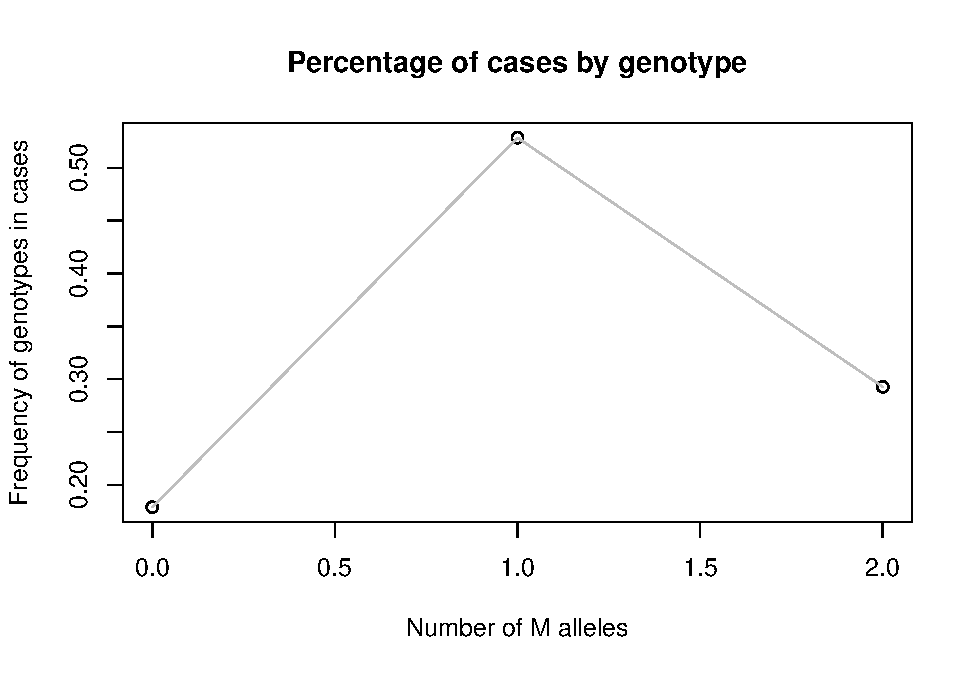
\includegraphics{P062020_Association_analysis_files/figure-latex/second-1.pdf}

Considering this plot, we can observe that the individuals with more
alleles \emph{M} has greater risk of disease than individuals with less
such alleles.

\begin{enumerate}
\def\labelenumi{\arabic{enumi}.}
\setcounter{enumi}{2}
\tightlist
\item
  (2p) Test for equality of allele frequencies in cases and controls by
  doing an alleles test. Report the test statistic, its reference
  distribution, and the p-value of the test. Is there evidence for
  different allele frequencies?
\end{enumerate}

\begin{Shaded}
\begin{Highlighting}[]
\NormalTok{mcases <-}\StringTok{ }\DecValTok{2}\OperatorTok{*}\KeywordTok{sum}\NormalTok{(data[,}\DecValTok{2}\NormalTok{] }\OperatorTok{==}\StringTok{ 'case'} \OperatorTok{&}\StringTok{ }\NormalTok{data[,}\DecValTok{1}\NormalTok{] }\OperatorTok{==}\StringTok{ 'mm'}\NormalTok{) }\OperatorTok{+}\StringTok{ }\KeywordTok{sum}\NormalTok{(data[,}\DecValTok{2}\NormalTok{] }\OperatorTok{==}\StringTok{ 'case'} \OperatorTok{&}\StringTok{ }\NormalTok{data[,}\DecValTok{1}\NormalTok{] }\OperatorTok{==}\StringTok{ 'Mm'}\NormalTok{)}
\NormalTok{Mcases <-}\StringTok{ }\DecValTok{2}\OperatorTok{*}\KeywordTok{sum}\NormalTok{(data[,}\DecValTok{2}\NormalTok{] }\OperatorTok{==}\StringTok{ 'case'} \OperatorTok{&}\StringTok{ }\NormalTok{data[,}\DecValTok{1}\NormalTok{] }\OperatorTok{==}\StringTok{ 'MM'}\NormalTok{) }\OperatorTok{+}\StringTok{ }\KeywordTok{sum}\NormalTok{(data[,}\DecValTok{2}\NormalTok{] }\OperatorTok{==}\StringTok{ 'case'} \OperatorTok{&}\StringTok{ }\NormalTok{data[,}\DecValTok{1}\NormalTok{] }\OperatorTok{==}\StringTok{ 'Mm'}\NormalTok{)}
\NormalTok{mcontrol <-}\StringTok{ }\DecValTok{2}\OperatorTok{*}\KeywordTok{sum}\NormalTok{(data[,}\DecValTok{2}\NormalTok{] }\OperatorTok{==}\StringTok{ 'control'} \OperatorTok{&}\StringTok{ }\NormalTok{data[,}\DecValTok{1}\NormalTok{] }\OperatorTok{==}\StringTok{ 'mm'}\NormalTok{) }\OperatorTok{+}\StringTok{ }\KeywordTok{sum}\NormalTok{(data[,}\DecValTok{2}\NormalTok{] }\OperatorTok{==}\StringTok{ 'control'} \OperatorTok{&}\StringTok{ }\NormalTok{data[,}\DecValTok{1}\NormalTok{] }\OperatorTok{==}\StringTok{ 'Mm'}\NormalTok{)}
\NormalTok{Mcontrol <-}\StringTok{ }\DecValTok{2}\OperatorTok{*}\KeywordTok{sum}\NormalTok{(data[,}\DecValTok{2}\NormalTok{] }\OperatorTok{==}\StringTok{ 'control'} \OperatorTok{&}\StringTok{ }\NormalTok{data[,}\DecValTok{1}\NormalTok{] }\OperatorTok{==}\StringTok{ 'MM'}\NormalTok{) }\OperatorTok{+}\StringTok{ }\KeywordTok{sum}\NormalTok{(data[,}\DecValTok{2}\NormalTok{] }\OperatorTok{==}\StringTok{ 'control'} \OperatorTok{&}\StringTok{ }\NormalTok{data[,}\DecValTok{1}\NormalTok{] }\OperatorTok{==}\StringTok{ 'Mm'}\NormalTok{)}

\NormalTok{allele_freq <-}\StringTok{ }\KeywordTok{rbind}\NormalTok{(}\KeywordTok{c}\NormalTok{(mcases, Mcases), }\KeywordTok{c}\NormalTok{(mcontrol, Mcontrol))}
\KeywordTok{colnames}\NormalTok{(allele_freq) <-}\StringTok{ }\KeywordTok{c}\NormalTok{(}\StringTok{"m"}\NormalTok{,}\StringTok{"M"}\NormalTok{)}
\KeywordTok{rownames}\NormalTok{(allele_freq) <-}\StringTok{ }\KeywordTok{c}\NormalTok{(}\StringTok{"Cases"}\NormalTok{, }\StringTok{"Control"}\NormalTok{)}
\NormalTok{(allele_freq)}
\end{Highlighting}
\end{Shaded}

\begin{verbatim}
##           m   M
## Cases   451 567
## Control 685 631
\end{verbatim}

\begin{Shaded}
\begin{Highlighting}[]
\KeywordTok{chisq.test}\NormalTok{(allele_freq,}\DataTypeTok{correct=}\OtherTok{FALSE}\NormalTok{)}
\end{Highlighting}
\end{Shaded}

\begin{verbatim}
## 
##  Pearson's Chi-squared test
## 
## data:  allele_freq
## X-squared = 13.797, df = 1, p-value = 0.0002037
\end{verbatim}

\begin{Shaded}
\begin{Highlighting}[]
\KeywordTok{fisher.test}\NormalTok{(allele_freq)}
\end{Highlighting}
\end{Shaded}

\begin{verbatim}
## 
##  Fisher's Exact Test for Count Data
## 
## data:  allele_freq
## p-value = 0.0002368
## alternative hypothesis: true odds ratio is not equal to 1
## 95 percent confidence interval:
##  0.6195641 0.8664957
## sample estimates:
## odds ratio 
##  0.7328195
\end{verbatim}

As the chi-squared statistic of \textbf{13.797} which corresponds to
p-value \textbf{0.0002037} exceeds the critical value, we reject the
null hypothesis and conclude that the allele frequencies are biased at
95\% significance level. We say that there is enough evidence for
different allele frequencies. Fisher's Exact Test gave very similar
results.

\begin{enumerate}
\def\labelenumi{\arabic{enumi}.}
\setcounter{enumi}{3}
\tightlist
\item
  (2p) Which are the assumptions made by the alleles test? Perform and
  report any additional tests you consider adequate to verify the
  assumptions. Do you think the assumptions of the alleles test are met?
\end{enumerate}

The assumptions made by chi-squared test are \textbf{random sampling},
\textbf{sufficiently large size of sample}, \textbf{expected cell count
greater than 5} and \textbf{independence of the observations}. The
chi-squared test also relies on HW equilibrium assumption. Sample size
seems sufficiently large and expected cell count is great enough. We
assume that observations are randomly sampled and independent. What left
is to check if the variant is in HW equilibrium.

\begin{Shaded}
\begin{Highlighting}[]
\NormalTok{genotypes <-}\StringTok{ }\KeywordTok{c}\NormalTok{(}\KeywordTok{sum}\NormalTok{(data[,}\DecValTok{1}\NormalTok{] }\OperatorTok{==}\StringTok{ 'mm'}\NormalTok{), }\KeywordTok{sum}\NormalTok{(data[,}\DecValTok{1}\NormalTok{] }\OperatorTok{==}\StringTok{ 'Mm'}\NormalTok{), }\KeywordTok{sum}\NormalTok{(data[,}\DecValTok{1}\NormalTok{] }\OperatorTok{==}\StringTok{ 'MM'}\NormalTok{))}
\KeywordTok{names}\NormalTok{(genotypes) <-}\StringTok{ }\KeywordTok{c}\NormalTok{(}\StringTok{"mm"}\NormalTok{,}\StringTok{"Mm"}\NormalTok{, }\StringTok{"MM"}\NormalTok{)}
\KeywordTok{HWChisq}\NormalTok{(genotypes)}
\end{Highlighting}
\end{Shaded}

\begin{verbatim}
## Chi-square test with continuity correction for Hardy-Weinberg equilibrium (autosomal)
## Chi2 =  0.3546387 DF =  1 p-value =  0.551499 D =  5.45587 f =  -0.0187137
\end{verbatim}

Considering p-value is greater than critical value, we can not reject
the null hypotesis which states that the variant is in equilibrium. So,
we think assumptions of the alleles test are met

\begin{enumerate}
\def\labelenumi{\arabic{enumi}.}
\setcounter{enumi}{4}
\tightlist
\item
  (2p) Perform the Armitage trend test for association between disease
  and number of M alleles. Report the test statistic, its reference
  distribution and the p-value of the test. Do you find evidence for
  association?
\end{enumerate}

\begin{Shaded}
\begin{Highlighting}[]
\NormalTok{x <-}\StringTok{ }\KeywordTok{as.integer}\NormalTok{(data[,}\DecValTok{2}\NormalTok{] }\OperatorTok{==}\StringTok{ 'case'}\NormalTok{)}
\NormalTok{y <-}\StringTok{ }\KeywordTok{sapply}\NormalTok{(data[,}\DecValTok{1}\NormalTok{], }\ControlFlowTok{function}\NormalTok{(x) }\KeywordTok{sum}\NormalTok{(}\KeywordTok{unlist}\NormalTok{(}\KeywordTok{strsplit}\NormalTok{(x, }\DataTypeTok{split =} \StringTok{""}\NormalTok{)) }\OperatorTok{==}\StringTok{ 'M'}\NormalTok{))}

\NormalTok{r <-}\StringTok{ }\KeywordTok{cor}\NormalTok{(x,y)}
\NormalTok{A <-}\StringTok{ }\NormalTok{n}\OperatorTok{*}\NormalTok{(r}\OperatorTok{^}\DecValTok{2}\NormalTok{)}

\NormalTok{pvalue <-}\StringTok{ }\KeywordTok{pchisq}\NormalTok{(A,}\DataTypeTok{df=}\DecValTok{1}\NormalTok{,}\DataTypeTok{lower.tail=}\OtherTok{FALSE}\NormalTok{)}
\KeywordTok{cat}\NormalTok{(}\KeywordTok{paste}\NormalTok{(}\StringTok{'p-value:'}\NormalTok{, pvalue))}
\end{Highlighting}
\end{Shaded}

\begin{verbatim}
## p-value: 0.000177091650268061
\end{verbatim}

Armitage trend test produced p-value of \textbf{0.000177091} which is
lower than critical p-value of \textbf{0.05}. We can reject the null
hypotesis and say that there exist a trend and enough evidence for
association.

\begin{enumerate}
\def\labelenumi{\arabic{enumi}.}
\setcounter{enumi}{5}
\tightlist
\item
  (4p) Test for association between genotype and disease status by a
  logistic regression of disease status on genotype, treating the latter
  as categorical. Do you find significant evidence for association?
  Which allele increase the risk for the disease? Give the odds ratios
  of the genotypes with respect to base line genotype mm. Provide 95\%
  confidence intervals for these odds ratios.
\end{enumerate}

\begin{Shaded}
\begin{Highlighting}[]
\NormalTok{y <-}\StringTok{ }\NormalTok{x}
\NormalTok{x <-}\StringTok{ }\KeywordTok{factor}\NormalTok{(data[,}\DecValTok{1}\NormalTok{])}

\NormalTok{out.lm <-}\StringTok{ }\KeywordTok{glm}\NormalTok{(y}\OperatorTok{~}\NormalTok{x, }\DataTypeTok{family =} \KeywordTok{binomial}\NormalTok{(}\DataTypeTok{link =} \StringTok{"logit"}\NormalTok{))}
\NormalTok{summ <-}\StringTok{ }\KeywordTok{summary}\NormalTok{(out.lm)}
\NormalTok{summ}
\end{Highlighting}
\end{Shaded}

\begin{verbatim}
## 
## Call:
## glm(formula = y ~ x, family = binomial(link = "logit"))
## 
## Deviance Residuals: 
##     Min       1Q   Median       3Q      Max  
## -1.1662  -1.0982  -0.9046   1.2587   1.4773  
## 
## Coefficients:
##             Estimate Std. Error z value Pr(>|z|)    
## (Intercept)  -0.6821     0.1286  -5.303 1.14e-07 ***
## xMm           0.4930     0.1528   3.227 0.001251 ** 
## xMM           0.6556     0.1726   3.798 0.000146 ***
## ---
## Signif. codes:  0 '***' 0.001 '**' 0.01 '*' 0.05 '.' 0.1 ' ' 1
## 
## (Dispersion parameter for binomial family taken to be 1)
## 
##     Null deviance: 1598.7  on 1166  degrees of freedom
## Residual deviance: 1582.7  on 1164  degrees of freedom
## AIC: 1588.7
## 
## Number of Fisher Scoring iterations: 4
\end{verbatim}

\begin{Shaded}
\begin{Highlighting}[]
\NormalTok{or <-}\StringTok{ }\KeywordTok{exp}\NormalTok{(summ}\OperatorTok{$}\NormalTok{coefficients[,}\DecValTok{1}\NormalTok{])}
\NormalTok{orl <-}\StringTok{ }\KeywordTok{exp}\NormalTok{(summ}\OperatorTok{$}\NormalTok{coefficients[,}\DecValTok{1}\NormalTok{] }\OperatorTok{-}\StringTok{ }\FloatTok{1.96}\OperatorTok{*}\NormalTok{summ}\OperatorTok{$}\NormalTok{coefficients[,}\DecValTok{2}\NormalTok{])}
\NormalTok{org <-}\StringTok{ }\KeywordTok{exp}\NormalTok{(summ}\OperatorTok{$}\NormalTok{coefficients[,}\DecValTok{1}\NormalTok{] }\OperatorTok{+}\StringTok{ }\FloatTok{1.96}\OperatorTok{*}\NormalTok{summ}\OperatorTok{$}\NormalTok{coefficients[,}\DecValTok{2}\NormalTok{])}

\KeywordTok{cat}\NormalTok{(}\KeywordTok{paste}\NormalTok{(}\StringTok{'Ratio of odds for diseas with Mm person and mm person: '}\NormalTok{, or[}\DecValTok{2}\NormalTok{], }\StringTok{' (95% confidence interval: ['}\NormalTok{, orl[}\DecValTok{2}\NormalTok{], }\StringTok{', '}\NormalTok{, org[}\DecValTok{2}\NormalTok{], }\StringTok{']}\CharTok{\textbackslash{}n}\StringTok{'}\NormalTok{, }\DataTypeTok{sep=}\StringTok{''}\NormalTok{))}
\end{Highlighting}
\end{Shaded}

\begin{verbatim}
## Ratio of odds for diseas with Mm person and mm person: 1.63719357565482 (95% confidence interval: [1.21355312605524, 2.20872308481317]
\end{verbatim}

\begin{Shaded}
\begin{Highlighting}[]
\KeywordTok{cat}\NormalTok{(}\KeywordTok{paste}\NormalTok{(}\StringTok{'Ratio of odds for diseas with MM person and mm person: '}\NormalTok{, or[}\DecValTok{3}\NormalTok{], }\StringTok{' (95% confidence interval: ['}\NormalTok{, orl[}\DecValTok{3}\NormalTok{], }\StringTok{', '}\NormalTok{, org[}\DecValTok{3}\NormalTok{], }\StringTok{']}\CharTok{\textbackslash{}n}\StringTok{'}\NormalTok{, }\DataTypeTok{sep=}\StringTok{''}\NormalTok{))}
\end{Highlighting}
\end{Shaded}

\begin{verbatim}
## Ratio of odds for diseas with MM person and mm person: 1.92630898513217 (95% confidence interval: [1.37341886551983, 2.70177321672109]
\end{verbatim}

As we can see from the output of \textbf{summmary} of \textbf{glm}
function, each one of the coefficients is significant and therefore
which is enough evidence for association between genotype and disease
status. We can also see the same results as from the plot in the second
task, telling that allel \textbf{M} increases the risk for the disease.

\end{document}
